%=============================================================
%  Bond-Graph Modelling of the UR5 Robot Manipulator
%  with PD + Gravity-Compensation Control
%=============================================================
\documentclass[12pt,a4paper,oneside]{report}

%--- packages ------------------------------------------------
\usepackage[T1]{fontenc}
\usepackage[utf8]{inputenc}
\usepackage[english]{babel}
\usepackage{geometry}
\geometry{margin=2.5cm}
\usepackage{amsmath,amssymb,amsfonts,bm}
\usepackage{graphicx}
\usepackage{float}
\usepackage{booktabs}
\usepackage{array}
\usepackage{multirow}
\usepackage{caption}
\usepackage{subcaption}
\usepackage{xcolor}
\usepackage{tikz}
\usepackage{pgfplots}
\pgfplotsset{compat=1.18}
\usepackage{hyperref}
\hypersetup{colorlinks=true, linkcolor=blue, citecolor=blue, urlcolor=blue}
\usepackage{listings}
\usepackage{enumitem}
\usepackage{tcolorbox}
\tcbuselibrary{skins,breakable}
\usepackage{fancyhdr}
\usepackage{titlesec}
\usepackage{cleveref}
\usepackage{titling}

%--- page style ---------------------------------------------
\pagestyle{fancy}
\fancyhf{}
\fancyhead[L]{\nouppercase{\leftmark}}
\fancyhead[R]{\thepage}
\renewcommand{\headrulewidth}{0.4pt}

%--- placeholder box style -----------------------------------
\newtcolorbox{placeholder}[1][]{
  enhanced, breakable,
  colback=gray!10, colframe=gray!60,
  fonttitle=\bfseries\small,
  title={#1},
  halign title=center,
  top=6pt, bottom=6pt,
  left=6pt, right=6pt,
}


%=============================================================
\begin{document}
%=============================================================



\thispagestyle{empty}                                                 
\begin{center}                                                            
    \vspace{5mm}
    {\LARGE UNIVERSIT\`A DI BOLOGNA} \\                       
      \vspace{5mm}
\end{center}
\begin{center}
  
\includegraphics[scale=.27]{figs/logo_unibo}
\end{center}
\begin{center}
      \vspace{5mm}
      {\Large Master's Degree in Automation Engineering} \\
      \vspace{20mm}
      {\LARGE Modeling and Simulation of Mechatronic Systems} \\
      \vspace{5mm}{\Large\textbf{UR5 ROBOT BOND GRAPH MODEL}} \\                 
      \vspace{15mm}
\end{center}


\begin{center}
      {\large Giulio Mazzaroppi, Francesco Cenni, Giacomo Pezzolati} \\
\end{center}


\begin{center}
\vfill
      {\large Academic year \@25/26} \\
\end{center}

\newpage
\thispagestyle{empty}



\tableofcontents

%=============================================================
\chapter{The Link Sub-Model}
\label{chap:link}
%=============================================================

\section{Physical Description}

Each link of the UR5 is modelled as a rigid body characterised by:
\begin{itemize}
  \item a mass $m$,
  \item an inertia tensor $J \in \mathbb{R}^{3\times3}$ expressed in the link frame,
  \item the position of the centre of mass $r_{Gp}$ with respect to the link's proximal joint frame origin.
\end{itemize}
Numerical values for the UR5, taken from \cite{Macchelli2026}, are listed in \cref{tab:link_params}.

\begin{table}[H]
  \centering
  \caption{UR5 link masses, centres of gravity, and diagonal inertia components.}
  \label{tab:link_params}
  \begin{tabular}{@{}ccccc@{}}
    \toprule
    Link & $m$ [kg] & $r_{Gp,x}$ [m] & $r_{Gp,y}$ [m] & $r_{Gp,z}$ [m] \\
    \midrule
    1 & 3.700  &  0.0000 & $-$0.02561 &  0.00193 \\
    2 & 8.393  &  0.2125 &  0.0000   &  0.11336 \\
    3 & 2.330  &  0.1500 &  0.0000   &  0.02650 \\
    4 & 1.1219 &  0.0000 & $-$0.00180 &  0.01634 \\
    5 & 1.1219 &  0.0000 &  0.00180  &  0.01634 \\
    6 & 0.1879 &  0.0000 &  0.0000   & $-$0.001159 \\
    \bottomrule
  \end{tabular}
\end{table}

\section{Ports and parameters}

\section{Equations of Motion}

The Newton--Euler equations for link $i$, written in the body frame attached to the link, are given by \cref{eq:newton,eq:euler}.
Denoting the generalised momentum as
\begin{equation}
  p_{\text{lin}} = m\,v_G, \qquad h_{\text{ang}} = J\,\omega,
\end{equation}
one obtains the state-space form that 20-sim integrates directly:
\begin{align}
  \dot{p}_{\text{lin}} &= f^{\text{ext}} + m\,\omega \times v_G, \\
  \dot{h}_{\text{ang}} &= \tau^{\text{ext}} + \omega \times J\omega, \\
  v_G &= p_{\text{lin}} / m, \\
  \omega &= J^{-1} h_{\text{ang}}.
\end{align}

\section{Bond-Graph Structure}

The \texttt{Link} sub-model exposes two \emph{power ports} of dimension six:
\begin{itemize}
  \item \texttt{wrench\_i}: the wrench applied at the proximal joint (input, integral causality).
  \item \texttt{wrench\_ipp}: the wrench at the distal joint (input, integral causality).
\end{itemize}
It also receives a signal input \texttt{T\_next}, the homogeneous transformation, used to orient gravity.

Internally the model contains:
\begin{enumerate}
  \item Two \textbf{MTF} elements (\texttt{i\_com} and \texttt{ipp\_com}) that shift the reference from the joint origins to the centre of mass via \cref{eq:vel_shift,eq:torque_shift}.
  \item A \textbf{1-junction} that enforces the common-velocity constraint at the centre of mass and sums all efforts.
  \item The \textbf{Body} I-element that integrates the Newton--Euler equations.
  \item A \textbf{MSe} element that injects the gravitational wrench.
\end{enumerate}

\subsection{Gravity Source (MSe)}

The gravitational force in the inertial frame is $f_g = [0,\,0,\,-mg]^T$.
To express it in the body frame of link $i$, the rotation matrix $R_i \in SO(3)$ extracted from \texttt{T\_next} is used:
\begin{equation}
  f_g^{\text{body}} = R_i^T \begin{pmatrix}0\\0\\-mg\end{pmatrix}, \qquad \tau_g^{\text{body}} = \mathbf{0}.
\end{equation}
This wrench is injected at the 1-junction so that it acts on the body mass.

\subsection{Body sub-model}

\subsection{MTF Equations}

For a displacement vector $r_{Gp} \in \mathbb{R}^3$ from the joint origin to the CoM:
\begin{align}
  v_G &= v_{\text{joint}} + \omega \times r_{Gp}, \\
  \tau_{\text{joint}} &= \tau_G + r_{Gp} \times f_G.
\end{align}
These equations are implemented as a modulated transformer in 20-sim, where the modulation matrix is $[r_{Gp}]_\times$.

\subsection{Causality Assignment}

Both power ports carry \emph{fixed integral causality} (the effort is known, the flow is computed).
This means:
\begin{itemize}
  \item Efforts (forces/torques at the joints) are \emph{given} by the connected joints.
  \item Velocities (flows) are \emph{computed} by the body integrator.
\end{itemize}
The 1-junction has one element with \emph{effort-out} causality (the Body I-element) and all others with \emph{effort-in} causality (the two MTF connections and the MSe source).
The \emph{constraint}: MTF elements with fixed causality on both sides impose a \emph{causality conflict} unless the effort-output side is consistently identified --- this is resolved by stipulating that the Body is the unique element on the 1-junction that imposes effort.

\begin{placeholder}[FIGURE PLACEHOLDER -- Link Bond-Graph Diagram]
  \centering
  \vspace{3cm}
  \textit{Insert here the bond-graph diagram of the \texttt{Link} sub-model, showing the two MTF elements connecting the proximal and distal joint ports to the 1-junction, the Body I-element, and the MSe gravity source.
  Causality strokes should be clearly indicated on each half-bond.}
  \vspace{3cm}
\end{placeholder}
%=============================================================
\chapter{The Joint Sub-Model}
\label{chap:joint}
%=============================================================

\section{Physical Description}

Each of the six joints of the UR5 is a revolute joint.
In the bond-graph model, the \texttt{Joint} sub-model is responsible for:
\begin{enumerate}
  \item Performing the DH frame transformation between the inbound and outbound twist ports.
  \item Extracting the scalar joint velocity $\dot{q}_i$ and position $q_i$.
  \item Receiving the scalar actuator torque $\tau_i$ and transmitting it to the mechanical chain.
\end{enumerate}

\section{Ports and Parameters}

\begin{table}[H]
  \centering
  \caption{\texttt{Joint} sub-model ports.}
  \begin{tabular}{@{}lll@{}}
    \toprule
    Port & Type & Description \\
    \midrule
    \texttt{twist\_i}    & power in  (fixed-out causality) & Twist of frame $i-1$ \\
    \texttt{twist\_ipp}  & power out (fixed-out causality) & Twist of frame $i$ \\
    \texttt{actuator}    & power in  (fixed-in causality)  & Actuator scalar torque bond \\
    \texttt{T\_i}        & signal out $[4\times4]$         & DH homogeneous transformation $H_i^{i-1}$ \\
    \texttt{Q}           & signal out $[2\times1]$         & Joint state $[q_i,\;\dot{q}_i]^T$ \\
    \bottomrule
  \end{tabular}
\end{table}

DH parameters stored in the \texttt{Joint} sub-model are $d_i$, $a_i$, $\alpha_i$, and the offset $\tilde{q}_i$.
These are set for each of the six joints according to \cref{tab:dh_params}.

\begin{table}[H]
  \centering
  \caption{UR5 Denavit--Hartenberg parameters.}
  \label{tab:dh_params}
  \begin{tabular}{@{}lccccc@{}}
    \toprule
    Joint & $d_i$ [m] & $a_i$ [m] & $\alpha_i$ [rad] & $\tilde{q}_i$ [rad] \\
    \midrule
    Base   (1) & 0.089159 &  0.0       & $\pi/2$   & 0 \\
    Shoulder(2)& 0.0      & $-$0.425   & 0         & 0 \\
    Elbow  (3) & 0.0      & $-$0.39225 & 0         & 0 \\
    Wrist1 (4) & 0.10915  &  0.0       & $\pi/2$   & 0 \\
    Wrist2 (5) & 0.09465  &  0.0       & $-\pi/2$  & 0 \\
    Wrist3 (6) & 0.0823   &  0.0       & 0         & 0 \\
    \bottomrule
  \end{tabular}
\end{table}

\section{The MTF Element as a DH Transformer}

The core of the \texttt{Joint} model is an MTF element that implements the DH transformation.
Given the joint angle $\theta_i = q_i + \tilde{q}_i$ and the stored parameters, the rotation matrix $R_i$ and translation $P_i$ are computed as follows (matching \cref{eq:dh}):
\begin{align}
  R_i &= \begin{pmatrix}
    \cos\theta_i & -\sin\theta_i\cos\alpha_i &  \sin\theta_i\sin\alpha_i \\
    \sin\theta_i &  \cos\theta_i\cos\alpha_i & -\cos\theta_i\sin\alpha_i \\
    0            &  \sin\alpha_i             &  \cos\alpha_i
  \end{pmatrix}, \\[6pt]
  P_i &= \begin{pmatrix}
    a_i\cos\theta_i \\ a_i\sin\theta_i \\ d_i
  \end{pmatrix}.
\end{align}
The MTF enforces power continuity by transforming twists and wrenches:
\begin{align}
  \tau_{\text{ipp}} &= R_i^T \tau_i, \\
  f_{\text{ipp}}    &= R_i^T f_i - R_i^T (P_i \times \tau_i), \\
  \omega_i          &= R_i\,\omega_{\text{ipp}}, \\
  v_i               &= P_i \times R_i\,\omega_{\text{ipp}} + R_i\,v_{\text{ipp}}.
\end{align}

\section{Joint Kinematics and Constraint Elements}

The joint variable $q_i$ (position) and $\dot{q}_i$ (velocity) are extracted from the power flow:
\begin{itemize}
  \item A \textbf{FlowSensor} reads the scalar rotational velocity $\dot{q}_i = \omega_z$ on the $z$-axis of frame $i-1$.
  \item An \textbf{Integrator} computes $q_i = \int \dot{q}_i\,dt$.
\end{itemize}
The joint imposes the revolute constraint: only rotation about $z$ is free.
This is achieved via:
\begin{itemize}
  \item A \textbf{ZeroJunction} for the $xy$-components of angular velocity (all equal and constrained to zero).
  \item A \textbf{ZeroJunction} for the $z$-component (free to rotate, actuated).
  \item A \textbf{0-junction} and constraint element (\texttt{Vel\_constr}, \texttt{Omega\_constr}) for translational and rotational velocities, enforcing that the joint is purely revolute.
\end{itemize}

\textbf{TODO: SPIEGARE MEGLIO CONSTRAINTS E REVOLUTE PAIR}


\section{Causality Assignment and Complexity}

The joint sub-model presents the most complex causality situation in the entire robot model:
\begin{itemize}
  \item The inbound port \texttt{twist\_i} has \emph{fixed effort-out} causality: the joint \emph{imposes} force/torque on the previous link and \emph{receives} velocity from it.
  \item The outbound port \texttt{twist\_ipp} has \emph{fixed effort-out} causality as well: the joint imposes force/torque on the next link.
  \item The MTF has a \emph{causality constraint}: the two sides must have opposite causality (one effort-in, one effort-out).
  \item The constraint elements (\texttt{Vel\_constr} for translational DoFs, \texttt{Omega\_constr} for $xy$-rotation) set effort from flow via an algebraic constraint equation, implying \emph{derivative causality} on the constrained directions.
  \item The \texttt{actuator} port has \emph{fixed-in causality}: the motor effort is imposed externally, so the 0-junction for $q_z$ has \emph{one effort-in} element (the actuator).
\end{itemize}

The combination of fixed causality on both external power ports and the internal MTF constraint means that \emph{no free integral causality} can be assigned to the internal inertia elements of the joint body; instead, these joints rely on the inertia of the connected links.
This is the correct physical interpretation: the joint itself has zero inertia in this model.

\begin{placeholder}[FIGURE PLACEHOLDER -- Joint Bond-Graph Diagram]
  \centering
  \vspace{3cm}
  \textit{Insert here the bond-graph diagram of the \texttt{Joint} sub-model.
  Show: the two power ports \texttt{twist\_i} and \texttt{twist\_ipp}, the central MTF implementing the DH transformation, the PowerDemux/PowerMux elements decomposing the 6-D twist into translational and rotational components, the 0-junctions and constraint blocks enforcing the revolute constraint, the FlowSensor and integrator extracting $\dot{q}_i$ and $q_i$, and the actuator bond.
  Causality strokes must be clearly marked.}
  \vspace{3cm}
\end{placeholder}
%=============================================================
\chapter{The Transformation Sub-Model}
\label{chap:transformation}
%=============================================================

\section{Role in the Kinematic Chain}

The \texttt{Transformation} sub-model is a \emph{signal-only} block that computes the cumulative homogeneous transformation from the previous frame $i-1$ to the current frame $i$. 

The transformation chain, as depicted in Figure \ref{fig:transformation_chain}, computes the total transformation with respect to the base frame, while also providing useful intermediate transformations.

\begin{figure}[H]
  \centering
  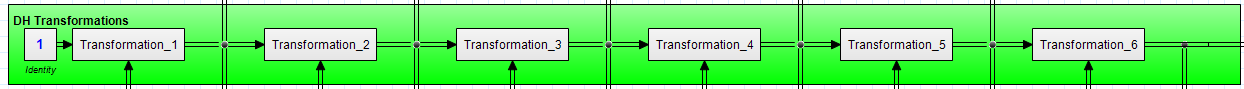
\includegraphics[width=1.0\textwidth]{chapter_transformation/figs/transformation_chain.png}
  \caption{Chain of transformations}
  \label{fig:transformation_chain}
\end{figure}

\section{Ports \& Parameters}
The \texttt{Transformation} sub-model's port structure is as follows:

\begin{center}
\begin{tikzpicture}[
    >=Stealth,
    every node/.style={font=\small},
    line width=0.8pt
]

\def\boxW{4.5}    % width of the black box
\def\boxH{2.2}    % height of the box
\def\arrowLen{2}  % length of arrows

\draw[fill=white, draw=black, line width=1.2pt]
    (0, -\boxH/2) rectangle (\boxW, \boxH/2);

\node[anchor=north, font=\normalsize\bfseries] at (\boxW/2, \boxH/2 - 0.2)
    {Transformation};

\draw[black, line width=0.5pt]
    (0.15, \boxH/2 - 0.7) -- (\boxW - 0.15, \boxH/2 - 0.7);

% DH Parameters
\node[anchor=north, font=\footnotesize, align=center] at (\boxW/2, \boxH/2 - 0.9)
    {$p_\text{body,i}$};

\def\yCentral{0}

% --- Input Signal Arrow (Left) ---
\draw[->, line width=1pt]
    (-\arrowLen, \yCentral) -- (0, \yCentral);
\node[above, font=\small] at (-\arrowLen/2, \yCentral + 0.05) {$\prescript{0}{}{T}_{i-1}$};

% --- Input Signal Arrow (Bottom) ---
\def\xBot{\boxW/2}
\draw[->, line width=1pt]
    (\xBot, -\boxH/2 - 1.5) -- (\xBot, -\boxH/2);
\node[right, font=\small] at (\xBot, -\boxH/2 - 0.75) {$\prescript{i-1}{}{T}_i$};

% --- Output Signal Arrow (Right) ---
\draw[->, line width=1pt]
    (\boxW, \yCentral) -- (\boxW + \arrowLen, \yCentral);
\node[above, font=\small] at (\boxW + \arrowLen/2, \yCentral + 0.05) {$\prescript{0}{}{T}_i$};

\end{tikzpicture}
\end{center}

The only given parameter is the position of the stl body with respect to the DH frame, denoted as $p_{\text{body}, i}$, which is used to offset the link body in the 3D visualization. The corresponding stl orientation is defined inside the \texttt{transformation} block.

\section{Equations}

Given the absolute transformation $\prescript{0}{}{T}_{i-1}$ up to frame $i-1$ and the incremental DH transformation $\prescript{i-1}{}{T}_i$ provided by the \texttt{Joint} block, the absolute transformation is updated as:
\begin{equation}
  \prescript{0}{}{T}_i = \prescript{0}{}{T}_{i-1} \cdot \prescript{i-1}{}{T}_i
  \label{eq:chain}
\end{equation}

The transformation from a general frame $i$ to the base frame is given by the product of the sequential transformations:
$$
\prescript{0}{}{T}_i = \prescript{0}{}{T}_1 \cdot \prescript{1}{}{T}_2 \dots \prescript{i-1}{}{T}_i 
$$

Furthermore, within each transformation block, the following variables are computed:

\begin{itemize}
  \item \textbf{Position of the DH frame with respect to the base frame:} $\prescript{0}{}{p}_i = T[1:3, 4]$, which is utilized to define the position of the DH frames in the 3D visualization. 
  \item \textbf{Orientation of the DH frame with respect to the base frame:} $\prescript{0}{}{R}_i = T[1:3, 1:3]$. This rotation matrix dictates the orientation of the DH frame in the 3D visualization and is also transposed to re-orient the gravity vector from the base frame to the DH frame within the \textbf{MSe} element of the \texttt{Link} block.
  \item \textbf{Position of a relative point on link $i$ with respect to the base frame:} $\prescript{0}{}{p}_{\text{body}, i} = \prescript{0}{}{R}_i \prescript{i}{}{p}_{\text{body}, i} + \prescript{0}{}{p}_i$, used to offset the link body inside the 3D visualization.
  \item \textbf{Orientation of link $i$ with respect to the base frame:} $\prescript{0}{}{R}_{\text{body}, i} = \prescript{0}{}{R}_i \prescript{i}{}{R}_{\text{body}, i}$, used to properly orient the link body in the 3D visualization.
\end{itemize}

Lastly, the complete transformation matrix $T_{\text{next}}$ is utilized inside the gravity compensation block to compute the directional axes $z_i$, the positions of the DH frames $p_i$, and the centers of mass $p_{\text{com}, i}$, all evaluated with respect to the base frame.
%=============================================================
\chapter{The Harmonic Drive Sub-Model}
\label{chap:harmonic}
%=============================================================

\section{Motivation}

Real robotic joints are not directly driven: a gearbox with a high reduction ratio sits between the motor shaft and the output link.
In the UR5, \emph{harmonic-drive} (strain-wave) gearboxes are used.
These components exhibit several non-ideal characteristics that significantly affect the closed-loop performance:
\begin{enumerate}
  \item High gear ratio with near-zero backlash.
  \item Non-linear torsional stiffness (the flex-spline deforms elastically).
  \item Viscous friction at the input shaft.
  \item Asymmetric Coulomb friction (static friction differs for positive and negative rotation).
  \item Motor rotor inertia reflected through the gear ratio.
\end{enumerate}

The harmonic drive datasheets (HFUS-14 and HFUS-20 series, see \cref{tab:hd14,tab:hd20}) supply the rated and peak torques, maximum speeds, and moment-of-inertia values used to set the model parameters.

\begin{table}[H]
  \centering
  \caption{HFUS-14 harmonic drive specifications (selected entries).}
  \label{tab:hd14}
  \begin{tabular}{@{}lcc@{}}
    \toprule
    Parameter & Ratio 50 & Ratio 100 \\
    \midrule
    Repeated peak torque $T_p$ [Nm] & 18 & 28 \\
    Average torque $T_a$ [Nm]       & 6.9 & 11 \\
    Rated torque $T_r$ [Nm]         & 5.4 & 7.8 \\
    Moment of inertia $J$ [$10^{-4}$ kg\,m$^2$] & \multicolumn{2}{c}{0.033--0.091} \\
    \bottomrule
  \end{tabular}
\end{table}

\begin{table}[H]
  \centering
  \caption{HFUS-20 harmonic drive specifications (selected entries).}
  \label{tab:hd20}
  \begin{tabular}{@{}lcc@{}}
    \toprule
    Parameter & Ratio 80 & Ratio 100 \\
    \midrule
    Repeated peak torque $T_p$ [Nm] & 74 & 82 \\
    Average torque $T_a$ [Nm]       & 47 & 49 \\
    Rated torque $T_r$ [Nm]         & 34 & 40 \\
    Moment of inertia $J$ [$10^{-4}$ kg\,m$^2$] & \multicolumn{2}{c}{0.193--0.404} \\
    \bottomrule
  \end{tabular}
\end{table}

\section{Ports and Parameters}


\section{Bond-Graph Structure}

The \texttt{HarmonicDrive} sub-model has:
\begin{itemize}
  \item \texttt{motor}: scalar power port input (motor torque + angular velocity).
  \item \texttt{harmonic\_drive}: scalar power port output (joint torque + output shaft velocity).
\end{itemize}

The topology is shown schematically in the bond graph below.
The key elements are:

\paragraph{Motor inertia (I element).}
The rotor inertia $J_{\text{rotor}}$ (default $8\times10^{-6}$~kg\,m$^2$) stores kinetic energy of the motor shaft:
\begin{equation}
  J\,\dot{\omega}_m = \tau_m - \tau_{\text{friction}} - \tau_{\text{elastic}}/N,
\end{equation}
where $\omega_m$ is the motor angular velocity and $N$ is the gear ratio (stored as negative to account for sign convention, default $N=-0.01$, i.e.\ ratio of 100).

\paragraph{Gear ratio (TF element).}
The transformer element with ratio $N$ enforces:
\begin{equation}
  \tau_m = N \, \tau_{\text{out}}, \qquad \omega_{\text{out}} = N \, \omega_m.
\end{equation}

\paragraph{Torsional stiffness (C element -- non-linear).}
The flex-spline introduces a piecewise-linear torsional compliance parameterised by three stiffness zones:
\begin{equation}
  \tau_s(\varphi) =
  \begin{cases}
    k_1\,\varphi & \text{if } \varphi \leq \varphi_1 = T_1/k_1, \\
    k_2(\varphi-\varphi_1) + T_1 & \text{if } \varphi_1 < \varphi < \varphi_2, \\
    k_3(\varphi-\varphi_2) + T_2 & \text{if } \varphi \geq \varphi_2,
  \end{cases}
\end{equation}
where $\varphi = \int(\omega_{\text{out}} - \omega_{\text{load}})\,dt$ is the elastic twist of the flex-spline, and $k_1 = 4700$, $k_2 = 6100$, $k_3 = 7100$~Nm/rad, $T_1 = 2$~Nm, $T_2 = 6.9$~Nm.

\paragraph{Viscous friction at motor shaft (R element).}
\begin{equation}
  \tau_{\text{visc}} = b_w\,\omega_m, \qquad b_w = 6.4\times10^{-4}\;\text{Nm\,s/rad}.
\end{equation}

\paragraph{Asymmetric Coulomb friction at output shaft (R element).}
Friction at the output shaft is modelled as a smooth approximation to the sign function:
\begin{equation}
  \tau_f(\omega) = \frac{b_{f,+} - b_{f,-}}{2} \cdot \frac{2}{\pi}\arctan(\omega) + (b_{f,+}+b_{f,-}),
\end{equation}
with $b_{f,+} = 0.008$~Nm and $b_{f,-} = -0.007$~Nm.
This formulation avoids numerical stiffness introduced by a discontinuous sign function while faithfully capturing the asymmetry.

\subsection{Causality Assignment}

The \texttt{motor} port is fixed \emph{effort-in}: the motor torque source imposes effort.
The \texttt{harmonic\_drive} port is fixed \emph{effort-out}: the transmission output imposes torque on the joint.
Within the sub-model:
\begin{itemize}
  \item The 1-junction at the motor shaft has the I-element as the \emph{effort-out} element (integral causality), and the TF and R elements as effort-in elements.
  \item The 0-junction at the output shaft is the sum point for the elastic and Coulomb friction torques.
  \item The C element is in integral causality: $\dot{\varphi} = f_C$, $e_C = \tau_s(\varphi)$.
\end{itemize}
The non-linear C element breaks the direct algebraic loop that would exist if a linear C were used in derivative causality.

\begin{placeholder}[FIGURE PLACEHOLDER -- Harmonic Drive Bond-Graph Diagram]
  \centering
  \vspace{3cm}
  \textit{Insert here the bond-graph diagram of the \texttt{HarmonicDrive} sub-model.
  Show the 1-junction at the motor shaft (connecting the motor source, the I-element for rotor inertia, the R-element for viscous damping, and the TF for gear ratio), the 0-junction at the output shaft (connecting the elastic C-element, the asymmetric friction R1-element, and the harmonic\_drive output port), and the inner 1-junction coupling the two.
  Causality strokes should be clearly indicated.}
  \vspace{3cm}
\end{placeholder}
%=============================================================
\chapter{The PD Controller Sub-Model}
\label{chap:pd}
%=============================================================

\section{Control Objective}

The objective of the controller is to drive the vector of joint positions
$q = [q_1,\ldots,q_6]^T \in \mathbb{R}^6$
to a desired constant configuration $q^* \in \mathbb{R}^6$, compensating for the gravitational torque so that the equilibrium is exact regardless of the robot posture.

\textbf{TODO: A cosa serve implementare un controllo}


\section{Control Law}

The control torque applied to each joint is:
\begin{equation}
  \tau_i = K_{p,i}(q_i^* - q_i) + K_{d,i}(\dot{q}_i^* - \dot{q}_i) + \tau_{g,i}(q),
  \label{eq:pd_law}
\end{equation}
where:
\begin{itemize}
  \item $K_{p,i}$ is the proportional gain,
  \item $K_{d,i}$ is the derivative gain,
  \item $\tau_{g,i}(q)$ is the gravity compensation torque for joint $i$ (see \cref{chap:gravity}).
\end{itemize}
In vector form, with the gain row-vector $K = [K_p^T, K_d^T]$ and the extended state error $e = [q^*-q;\;\dot{q}^*-\dot{q}]$:
\begin{equation}
  \tau = K\,e + \tau_g.
  \label{eq:pd_vec}
\end{equation}
For a constant reference ($\dot{q}^* = 0$), the derivative term acts as pure damping injection.

\section{Bond-Graph Implementation}

Each \texttt{PD} block controls \emph{one joint}.
It receives:
\begin{itemize}
  \item the signal \texttt{Q} = $[q_i, \dot{q}_i]^T$ from the joint,
  \item the gravity torque \texttt{gravity} = $\tau_{g,i}$ from the \texttt{GravityTerm} block.
\end{itemize}
It outputs a scalar signal \texttt{tau} which is fed to the \texttt{actuator} port of the joint (or, when the harmonic drive is present, to the motor effort source).

Internally the block implements \cref{eq:pd_law} using:
\begin{enumerate}
  \item A \textbf{Constant} block outputting $q^*_{\text{ref}} = [q_i^*;\;0]^T$.
  \item A \textbf{PlusMinus} subtractor computing the error $e = q^*_{\text{ref}} - Q$.
  \item A \textbf{Gain} block multiplying by $K = [K_p, K_d]$.
  \item A second \textbf{PlusMinus} block subtracting the gravity term from the PD output:
    \begin{equation}
      \tau = K\,e - \tau_g.
    \end{equation}
    Note the subtraction sign: the gravity term is computed with the convention that gravity is a load torque to be cancelled, so the compensation adds it with the appropriate sign.
\end{enumerate}

\begin{placeholder}[FIGURE PLACEHOLDER -- PD + Gravity Compensation Block Diagram]
  \centering
  \vspace{2.5cm}
  \textit{Insert here the signal-flow block diagram of the \texttt{PD} sub-model.
  Show the constant reference block, the subtraction node producing the error $e = q^* - Q$, the gain matrix $K$ producing $K\,e$, and the second summation node where the gravity feedforward $\tau_g$ is added.
  Also indicate the signal connections to and from the joint state port \texttt{Q} and the gravity signal \texttt{gravity}.}
  \vspace{2.5cm}
\end{placeholder}

\section{Gravity compensation}
\subsection{Closed-Form Gravity Torque}

The gravity torque at joint $i$ is derived from the potential energy of all links $j \geq i$:
\begin{equation}
  \tau_{g,i} = \sum_{j=i}^{6} m_j\, g^T \left(z_{i-1} \times (p_{G,j}^0 - p_{i-1}^0)\right),
  \label{eq:gravity}
\end{equation}
where:
\begin{itemize}
  \item $g = [0,0,-9.81]^T$ m/s$^2$ is the gravity vector in the world frame,
  \item $z_{i-1}$ is the unit vector along the $z$-axis of frame $i-1$ expressed in world coordinates (the third column of the rotation part of $H_{i-1}$),
  \item $p_{G,j}^0$ is the position of the centre of mass of link $j$ in world coordinates,
  \item $p_{i-1}^0$ is the origin of frame $i-1$ in world coordinates.
\end{itemize}

\subsection{Implementation in the GravityTerm Block}

The \texttt{GravityTerm} block receives the six absolute transformations $H_1$ through $H_6$ as signal inputs (each $4\times4$) and outputs the six gravity compensation torques $\tau_g \in \mathbb{R}^6$.

For each joint $i$, the positions $p_j^0$ and $p_{G,j}^0$ are computed as:
\begin{align}
  p_j^0      &= H_j[1\!:\!3,4], \\
  p_{G,j}^0  &= H_j[1\!:\!3,1\!:\!3]\,r_{Gp,j} + p_j^0,
\end{align}
and the joint axis direction is:
\begin{equation}
  z_{i-1} = H_{i-1}[1\!:\!3,3].
\end{equation}
The torque \eqref{eq:gravity} is then evaluated numerically.

The \texttt{GravityTerm} block is a pure \emph{signal} block: it has no power ports and does not participate in the causality analysis of the bond graph.
Its outputs feed the six \texttt{PD} sub-models.

\begin{placeholder}[FIGURE PLACEHOLDER -- GravityTerm Signal Block Diagram]
  \centering
  \vspace{2cm}
  \textit{Insert here a signal-flow diagram of the \texttt{GravityTerm} block showing the six $4\times4$ transformation matrices arriving as inputs, the intermediate computations of $p_j^0$, $p_{G,j}^0$, $z_{i-1}$, and the cross-product summation producing each $\tau_{g,i}$.}
  \vspace{2cm}
\end{placeholder}
%=============================================================
\chapter{Overall Robot Architecture}
\label{chap:robot}
%=============================================================

\section{Hierarchical Structure}

The complete \texttt{Robot} model assembles the sub-models described in the previous chapters into a hierarchical structure. Figure \ref{fig:robot_arch} provides a conceptual overview of the interconnections.

\begin{figure}[H]
  \centering
  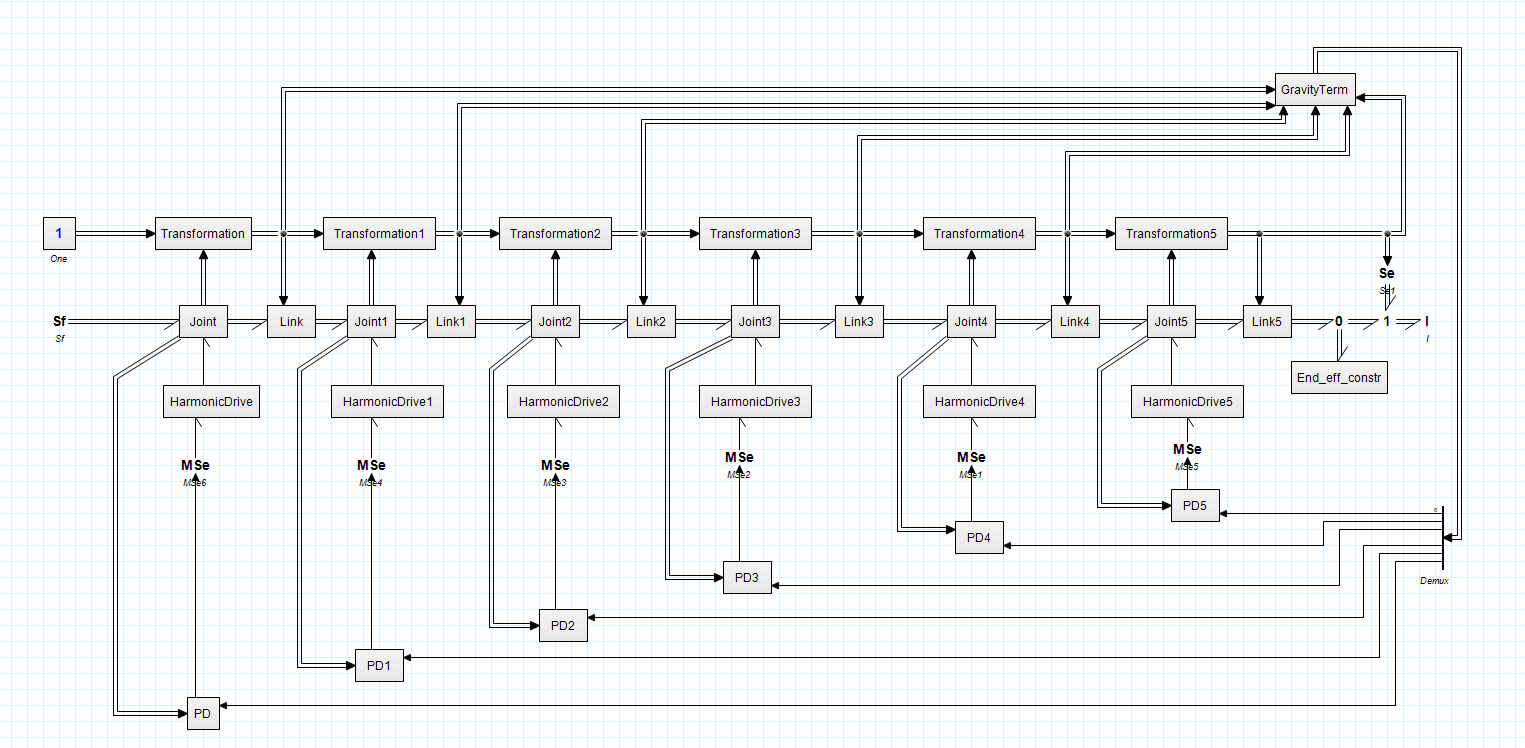
\includegraphics[width=1.0\textwidth]{chapter_robot/figs/robot_struct.png}
  \caption{Full robot architecture.}
  \label{fig:robot_arch}
\end{figure}

\section{Kinematic Chain Assembly}

\subsection{Robot Unit}
The robot comprises identical units consisting of the Joint, Link, Transformation, Harmonic Drive, and a PD controller with gravity compensation, all interconnected sequentially.

\begin{figure}[H]
  \centering
  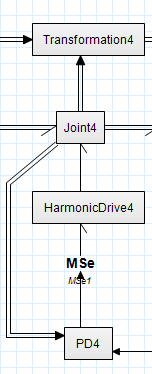
\includegraphics[width=0.3\textwidth]{chapter_robot/figs/robot_unit.png}
  \caption{Robot unit architecture.}
  \label{fig:robot_unit}
\end{figure}

\subsection{Power Bond Chain}

The mechanical power flows from the base (world frame, fixed) through the joints and links in sequence. The base is connected to a \emph{world bond}: a fixed-velocity source that sets the inertial frame velocity to zero ($S_f = 0$ for all six components).

For each link $i = 1,\ldots,6$, the connectivity is defined as:
\begin{center}
  Joint$_i$ (\texttt{twist\_ipp}) $\longrightarrow$ Link$_i$ (\texttt{wrench\_i})
  $\longrightarrow$ Link$_i$ (\texttt{wrench\_ipp}) $\longrightarrow$ Joint$_{i+1}$ (\texttt{twist\_i}).
\end{center}
After Joint$_6$ and Link$_6$, the distal power port terminates either in a free end (zero-force source) or within the payload model.

\subsection{Signal Chain for Transformations}

The absolute transformation chain initializes with $T_0 = I_4$ (the identity matrix, representing the world frame).
\begin{center}
  $T_0$ $\xrightarrow{\text{T\_prev}}$ Transf.$_1$ $\xrightarrow{\text{T\_next}=T_1}$ Transf.$_2$ $\xrightarrow{T_2}$ $\cdots$ $\xrightarrow{T_6}$ GravityTerm.
\end{center}
Each \texttt{Transformation} block also routes \texttt{T\_next} to the \texttt{MSe} element of the corresponding \texttt{Link} block (for gravity vector orientation) and to the 3D visualization.


\section{Global Causality Analysis}

The Link sub-model acts as an \textbf{I-field} in integral causality; therefore, its outputs at both ports are flows. This matches the causality of the Joint sub-model, which instead outputs effort from both ports. 

Consequently, the Joint block imposes the effort onto the robot chain, while the Links (representing the inertias) define the resulting velocities in response to this effort. 

To manage these computational constraints: 
\begin{itemize}
  \item The world bond imposes velocity (effort-out causality at the base).
  \item At the base, a source of flow ($S_f = 0$) simulates a stationary ground.
  \item At the end-effector (a Link), it is possible to attach either a source of effort to simulate a contact force, or an additional inertia with gravity to simulate a load.
  \item The harmonic drive outputs an effort, simulating a mechanical transmission. 
  \item The motor driving the shaft is simulated as a source of effort.
\end{itemize}

Moreover, the non-linear C-element within the harmonic drive retains integral causality. No derivative causality is present in the final assembled model, ensuring the numerical stability of the constrained integration via BDF solvers. 

\section{Payload Model}

A point-mass payload $m_{\text{load}}$ attached at the end-effector (the distal port of Link 6) is modeled as an additional \texttt{Link} block with:
\begin{itemize}
  \item $m = m_{\text{load}}$.
  \item $J = J_{\text{load}}$.
  \item $r_{Gp} = [0,0,0]^T$ (mass concentrated at the attachment point).
\end{itemize}

Gravity is also applied to its center of mass, which corresponds to the origin of the end-effector. This gravity vector is properly rotated according to the DH transformation of the end-effector frame. 

Lastly, to ensure a rigid connection between the final link and the payload, a zero-junction with a velocity constraint is employed in the exact same manner as in the Joint sub-model. 

\begin{figure}[H]
  \centering
  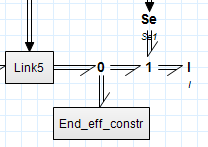
\includegraphics[width=0.4\textwidth]{chapter_robot/figs/load.png}
  \caption{Mass load architecture.}
  \label{fig:load_arch}
\end{figure}


\section{3-D Visualization}

The 20-sim 3-D Mechanics toolbox receives the pose signals (\texttt{pose\_abs}) and the rotation matrices from each \texttt{Transformation} block. STL bodies based on the UR5 model are utilized to represent each link. These bodies are positioned and oriented dynamically according to the offset positions and rotation matrices computed within the transformation blocks. 

\begin{figure}[H]
  \centering
  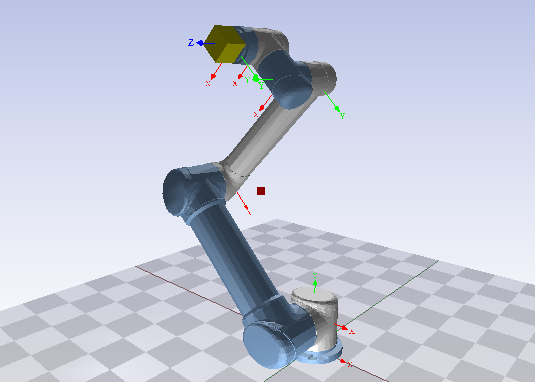
\includegraphics[width=0.8\textwidth]{chapter_robot/figs/stl1.png}
  \caption{Robot 3D visualization.}
  \label{fig:robot_visu}
\end{figure}
%=============================================================
\chapter{Simulation Results}
\label{chap:results}
%=============================================================

\section{Test Scenario}

The simulation is designed to test all layers of the model simultaneously:
\begin{enumerate}
  \item \textbf{Multi-joint step reference}: each joint is commanded to move from its initial angle to a specified target angle (mimicking a pick-and-place move).
  \item \textbf{Gravity compensation}: the arm must hold its posture against gravity at all times.
  \item \textbf{Harmonic drive effects}: the elastic flex-spline introduces a slight lag between the commanded and actual joint position.
  \item \textbf{Payload}: a 1~kg point mass is attached at the tool-centre point.
\end{enumerate}

The reference joint angles and PD gains used in the test are summarised in \cref{tab:test_params}.

\begin{table}[H]
  \centering
  \caption{Reference joint angles and PD gains for the test scenario.}
  \label{tab:test_params}
  \begin{tabular}{@{}ccccc@{}}
    \toprule
    Joint & $q^*$ [rad] & $\dot{q}^*$ [rad/s] & $K_p$ [Nm/rad] & $K_d$ [Nm\,s/rad] \\
    \midrule
    1 & 0.0   & 0 & 100 & 20 \\
    2 & $-\pi/4$ & 0 & 200 & 30 \\
    3 & $\pi/3$  & 0 & 150 & 25 \\
    4 & 0.0   & 0 & 80  & 15 \\
    5 & $\pi/6$  & 0 & 80  & 15 \\
    6 & 0.0   & 0 & 50  & 10 \\
    \bottomrule
  \end{tabular}
\end{table}

\section{3-D Animation}

\Cref{fig:anim1,fig:anim2,fig:anim3} show three snapshots from the 3-D animation: the initial configuration ($t=0$~s), mid-motion ($t\approx1.5$~s), and the final settled configuration ($t=5$~s).

\begin{figure}[H]
  \centering
  \begin{placeholder}[FIGURE PLACEHOLDER -- 3-D Animation Snapshot at $t = 0$ s (Initial Configuration)]
    \centering
    \vspace{3.5cm}
    \textit{Screenshot of the 20-sim 3-D animation at $t=0$~s.
    The robot is in its home position: all joint angles are zero.
    The arm hangs vertically.
    The payload (red sphere) is visible at the end-effector.}
    \vspace{3.5cm}
  \end{placeholder}
  \caption{3-D animation snapshot at $t=0$~s: initial (home) configuration.}
  \label{fig:anim1}
\end{figure}

\begin{figure}[H]
  \centering
  \begin{placeholder}[FIGURE PLACEHOLDER -- 3-D Animation Snapshot at $t \approx 1.5$ s (Mid-Motion)]
    \centering
    \vspace{3.5cm}
    \textit{Screenshot of the 20-sim 3-D animation at $t \approx 1.5$~s.
    Joints~2, 3, and 5 are visibly in motion; the arm is transitioning towards the target posture.
    Transient oscillation due to harmonic-drive compliance is evident.}
    \vspace{3.5cm}
  \end{placeholder}
  \caption{3-D animation snapshot at $t\approx1.5$~s: mid-motion transient.}
  \label{fig:anim2}
\end{figure}

\begin{figure}[H]
  \centering
  \begin{placeholder}[FIGURE PLACEHOLDER -- 3-D Animation Snapshot at $t = 5$ s (Final Settled Configuration)]
    \centering
    \vspace{3.5cm}
    \textit{Screenshot of the 20-sim 3-D animation at $t=5$~s.
    The arm has reached the target joint angles.
    The payload hangs at rest at the desired end-effector position.}
    \vspace{3.5cm}
  \end{placeholder}
  \caption{3-D animation snapshot at $t=5$~s: steady-state configuration.}
  \label{fig:anim3}
\end{figure}

\textbf{TODO: mettere video}

\section{Joint Position Tracking}

\Cref{fig:joint_pos} shows the time evolution of all six joint angles $q_i(t)$ compared to their references $q_i^*$.

\begin{figure}[H]
  \centering
  \begin{placeholder}[FIGURE PLACEHOLDER -- Joint Position Tracking Plots]
    \centering
    \vspace{5cm}
    \textit{A $2\times3$ subplot grid showing $q_i(t)$ (solid blue) vs.\ $q_i^*$ (dashed red) for $i = 1,\ldots,6$.
    Time axis: 0--5~s.
    Each subplot labelled ``Joint $i$''.
    Axes: $x$-axis time [s], $y$-axis angle [rad].
    Key features to show: smooth exponential approach to reference, slight overshoot on joints~2--3 (heavier links), fast convergence on joints~4--6 (lighter wrist).}
    \vspace{5cm}
  \end{placeholder}
  \caption{Joint position tracking: actual $q_i(t)$ (blue) vs.\ reference $q_i^*$ (red dashed).}
  \label{fig:joint_pos}
\end{figure}

\paragraph{Observation.}
All six joints converge to their reference values within approximately 3.5~s.
Joints~2 and~3, which carry the highest inertial and gravitational loads, show a small overshoot of roughly 3--5\%, consistent with the moderate derivative gain chosen.
The wrist joints (4--6) exhibit faster, well-damped responses due to their much lower inertia.

\section{Joint Torques}

\Cref{fig:joint_torque} shows the commanded torques $\tau_i(t)$ for all joints.

\begin{figure}[H]
  \centering
  \begin{placeholder}[FIGURE PLACEHOLDER -- Joint Torque Plots]
    \centering
    \vspace{5cm}
    \textit{A $2\times3$ subplot grid showing $\tau_i(t)$ for $i = 1,\ldots,6$ over 0--5~s.
    Axes: $x$-axis time [s], $y$-axis torque [Nm].
    Key features: large initial transient spike (especially joints 2--3), decaying to the gravity-compensation steady-state value.
    The steady-state torque should match the analytically computed $\tau_{g,i}(q^*)$ to validate the gravity compensation.}
    \vspace{5cm}
  \end{placeholder}
  \caption{Joint control torques $\tau_i(t)$ (blue: total; dashed orange: gravity feedforward component).}
  \label{fig:joint_torque}
\end{figure}

\paragraph{Observation.}
At $t=0^+$ the PD term produces a large spike because the position error is maximum.
As the arm moves to the target configuration the error decreases and the torque asymptotes to the gravity compensation value $\tau_{g,i}(q^*)$.
The close match between the steady-state commanded torque and the analytically predicted gravity torque confirms that the compensation term is correctly implemented.

\section{Harmonic Drive Elastic Deflection}

\Cref{fig:hd_deflection} shows the elastic twist $\varphi_i = q_{m,i}/N - q_i$ in the flex-spline of each harmonic drive.

\begin{figure}[H]
  \centering
  \begin{placeholder}[FIGURE PLACEHOLDER -- Harmonic Drive Elastic Deflection Plots]
    \centering
    \vspace{4cm}
    \textit{A $2\times3$ subplot grid showing the elastic deflection $\varphi_i(t)$ [mrad] for joints $i=1,\ldots,6$.
    Time axis: 0--5~s.
    Key features: peak deflection during initial transient, settling to near-zero at steady state.
    The non-linear stiffness characteristic causes slight asymmetry between positive and negative deflections.
    The piecewise character of the $k_1$--$k_2$--$k_3$ stiffness model may be visible as a slope change around $T_1$ and $T_2$.}
    \vspace{4cm}
  \end{placeholder}
  \caption{Elastic twist deflection $\varphi_i(t)$ in the harmonic drive flex-spline.}
  \label{fig:hd_deflection}
\end{figure}

\paragraph{Observation.}
Peak deflections occur during the transient and are bounded well within the rated torque limits of the selected HFUS-14/HFUS-20 units.
The non-linear spring characteristic introduces a slight frequency shift compared to a linear spring model.


%=============================================================
\section{Conclusions}
%=============================================================

A complete bond-graph model of the UR5 six-degree-of-freedom robot manipulator has been presented and validated.
Starting from the fundamental Newton--Euler equations of a rigid body expressed in terms of twists and wrenches, a hierarchical set of reusable 20-sim sub-models --- \texttt{Link}, \texttt{Joint}, \texttt{Transformation}, \texttt{HarmonicDrive}, \texttt{PD}, and \texttt{GravityTerm} --- was developed.

The following aspects deserve particular emphasis:
\begin{itemize}
  \item The \textbf{modulated transformer} (MTF) is the central bond-graph element for both the change-of-reference-point in the Link model and the DH transformation in the Joint model.
  \item \textbf{Causality assignment} is the most challenging design step: the dual fixed-causality constraint on the Joint power ports propagates through the chain and must be resolved without derivative causality by ensuring that the I-elements in the Link bodies are the only sources of differential equations.
  \item The \textbf{non-linear harmonic drive} C-element avoids the algebraic loop problem that would arise with a linear spring in derivative causality.
  \item The \textbf{GravityTerm} block, while signal-only, is critical for controller stability: without feedforward compensation, the PD controller cannot hold arbitrary postures.
  \item The \textbf{energy balance} validation, unique to bond-graph modelling, provides a powerful consistency check not available in equation-based formulations.
\end{itemize}

Future extensions could include: flexible link dynamics modelled with additional C-I chain elements; joint-space friction identification via parameter estimation; and extension to the complete UR10 or UR16e platforms using the same sub-model library.


\end{document}
